%!TeX root=../tempestrackham.tex

\Act*{1}
\Scene*{1}[On a ship at sea: a tempestuous noise of thunder and lightning heard.]

\begin{figure}[t]
	\centering
	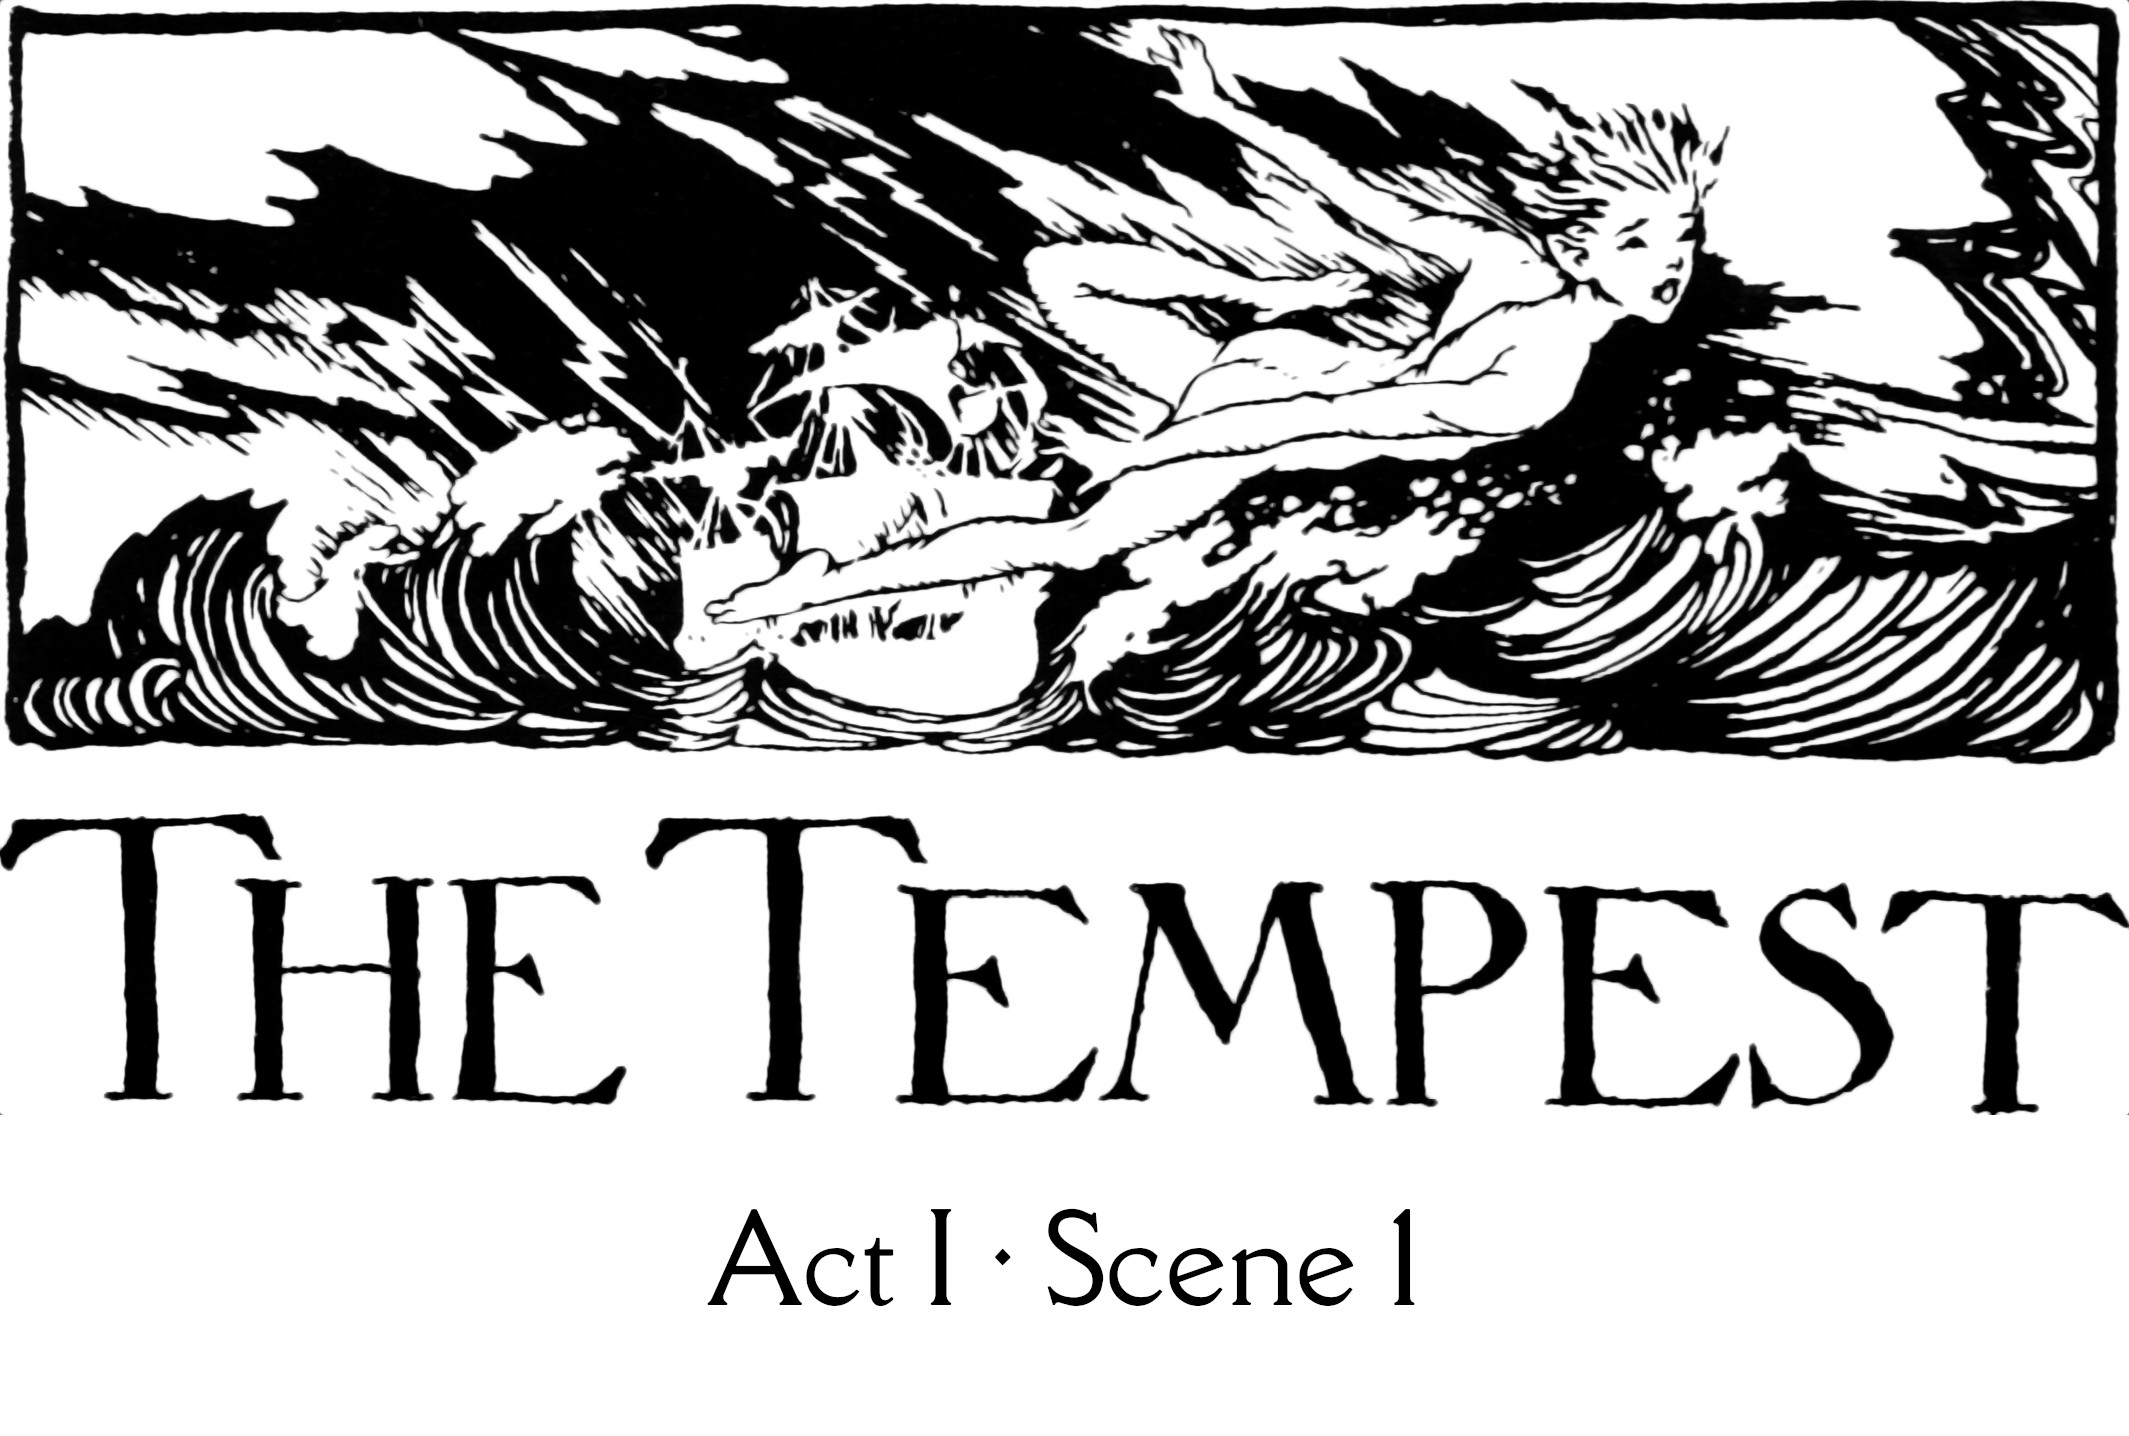
\includegraphics[width=\textwidth]{1ihead}
\end{figure}

\begin{letter}

\end{letter}

\vspace{\textsink}

\textit{(On a ship at sea: a tempestuous noise of thunder and lightning heard.)}\centering
\enter{a \textsc{Master} and a \textsc{Boatswain}}

\verseline[Master]{Boatswain!}
\verseline[Boatswain]{Here, master: what cheer?}
\verseline[Master]{Good, speak to the mariners: fall to't, yarely, or we run ourselves aground: bestir, bestir.}

\begin{prose_speech}[Boatswain] Heigh, my hearts! cheerly, cheerly, my hearts! yare, yare! Take in the topsail. Tend to the master's whistle. Blow, till thou burst thy wind, if room enough!
\end{prose_speech}

\enter{\textsc{Alonso}, \textsc{Sebastian}, \textsc{Antonio}, \textsc{Ferdinand}, \textsc{Gonzalo}, and others}

\begin{prose_speech}[Alonso] Good boatswain, have care. Where's the master? Play the men.
\end{prose_speech}


\begin{prose_speech}[Boatswain] I pray now, keep below.\end{prose_speech}

\begin{prose_speech}[Antonio] Where is the master, boatswain?\end{prose_speech}

\begin{prose_speech}[Boatswain] Do you not hear him? You mar our labour: keep your cabins: you do assist the storm.
\end{prose_speech}

\begin{prose_speech}[Gonzalo] Nay, good, be patient.\end{prose_speech}

\begin{prose_speech}[Boatswain] When the sea is. Hence! What cares these roarers for the name of king? To cabin: silence! trouble us not.\end{prose_speech}

\begin{prose_speech}[Gonzalo] Good, yet remember whom thou hast aboard.\end{prose_speech}

\begin{letter}
	\enlargethispage{\baselineskip}
\end{letter}
\begin{prose_speech}[Boatswain] None that I more love than myself. You are a counsellor; if you can command these elements to silence, and work the peace of the present, we will not hand a rope more; use your authority: if you cannot, give thanks you have lived so long, and make yourself ready in your cabin for the mischance of the hour, if it so hap. Cheerly, good hearts! Out of our way, I say.
\end{prose_speech}

\exit{\textsc{Boatswain}}

\begin{prose_speech}[Gonzalo] I have great comfort from this fellow: methinks he hath no drowning mark upon him; his complexion is perfect gallows. Stand fast, good Fate, to his hanging: make the rope of his destiny our cable, for our own doth little advantage. If he be not born to be hanged, our case is miserable.
\end{prose_speech}

\exit{\textsc{Gonzalo}, with \textsc{Alonso}, \textsc{Sebastian}, and the other courtiers.}


\enter{\textsc{Boatswain}}

\begin{prose_speech}[Boatswain] Down with the topmast! yare! lower, lower! Bring her to try with main-course.
\stage{A cry within}
A plague upon this howling! they are louder than the weather or our office.
\stage{Re-enter \textsc{Sebastian}, \textsc{Antonio}, and \textsc{Gonzalo}}
Yet again! what do you here? Shall we give o'er and drown? Have you a mind to sink?
\end{prose_speech}

\begin{prose_speech}[Sebastian] A pox o' your throat, you bawling, blasphemous, incharitable dog!
\end{prose_speech}

\begin{prose_speech}[Boatswain] Work you then.
	\end{prose_speech}

\begin{prose_speech}[Antonio] Hang, cur! hang, you whoreson, insolent noisemaker! We are less afraid to be drowned than thou art.
\end{prose_speech}

\begin{prose_speech}[Gonzalo] I'll warrant him for drowning; though the ship were no stronger than a nutshell and as leaky as an unstanched wench.
\end{prose_speech}

\begin{prose_speech}[Boatswain] Lay her a-hold, a-hold! set her two courses off to sea again; lay her off.
\end{prose_speech}

\enter{\textsc{Mariners} wet}

\begin{prose_speech}[Mariners] All lost! to prayers, to prayers! all lost!
	\end{prose_speech}

\exit{\textsc{Mariners}}

\begin{prose_speech}[Boatswain] What, must our mouths be cold?
	\end{prose_speech}

\begin{verse_speech}[Gonzalo] The king and prince at prayers! let's assist them,\\ For our case is as theirs.
\end{verse_speech}

\begin{verse_speech}[Sebastian] \hspace{\widthof{For our case is as theirs.}}I'm out of patience.\end{verse_speech}

\begin{verse_speech}[Antonio] We are merely cheated of our lives by drunkards:\\
This wide-chapp'd rascal—would thou mightst lie drowning\\
The washing of ten tides!\end{verse_speech}

\exit{\textsc{Boatswain}}

\begin{verse_speech}[Gonzalo] \hspace{\widthof{The washing of ten tides!}}He'll be hang'd yet,\\
Though every drop of water swear against it\\
And gape at widest to glut him.
\end{verse_speech}

\stage{A confused noise within: <Mercy on us!>—<We split, we split!>—<Farewell, my wife and children!>—<Farewell, brother!>—<We split, we split, we split!>}


\begin{verse_speech}[Antonio] Let's all sink with the king.\end{verse_speech}

\begin{verse_speech}[Sebastian] Let's take leave of him.\end{verse_speech}

\exit{\textsc{Antonio} and \textsc{Sebastian}}

\begin{prose_speech}[Gonzalo] Now would I give a thousand furlongs of sea for an acre of barren ground, long heath, brown furze, any  thing. The wills above be done! but I would fain die a dry death.
\end{prose_speech}

\exeunt{}

\begin{figure}[b]
	\centering
	
\includegraphics[width=\textwidth]{fish}
\end{figure}

